\documentclass{article}
\usepackage[margin=1in]{geometry}
\usepackage{amsmath}
\usepackage{amssymb}
\usepackage{graphicx}
\usepackage{cancel}
\usepackage{titlesec} %titleformat
\usepackage{enumerate} %for lists
\setlength{\parindent}{0em} %for vanish extra gap before paragraph
%\usepackage{etoolbox} %for patchcmd{}
%\patchcmd{\subequations}{{0}}{{-1}}{}{} %subequations iteration
%\patchcmd{\subequations}{\alph}{.\arabic}{}{} %setting subequations to decimal number
%\newcounter{cnt} %declaring a counter
%\newcommand\scnt{\stepcounter{cnt}\thecnt} %counter increment func
\usepackage{color}   %May be necessary if you want to color links
\usepackage{hyperref}
\hypersetup{
    colorlinks=true, %set true if you want colored links
    linktoc=all,     %set to all if you want both sections and subsections linked
    linkcolor=blue,  %choose some color if you want links to stand out
    %linktocpage     %for linking the page number only
}
\renewcommand{\baselinestretch}{1.5}%for space between two line
\pagestyle{myheadings}
\usepackage{pdfpages}


\begin{document}

\includepdf[pages=-]{cover.pdf}


\thispagestyle{empty}
\Large{\tableofcontents}
\thispagestyle{empty}
\newpage
\setcounter{page}{1}


%title format for sections
\titleformat{\section}
{\Large\bfseries}
{\thesection.}
{.5em}
{}[\titlerule]

%title format for subsections
\titleformat{\subsection}
{\Large\bfseries}
{(\thesubsection)}
{0em}
{}
\renewcommand\thesubsection{\alph {subsection}}

\section{Heart Attack}
\subsection{}%1.a
%\begin{figure}[h]
%    \centering
%    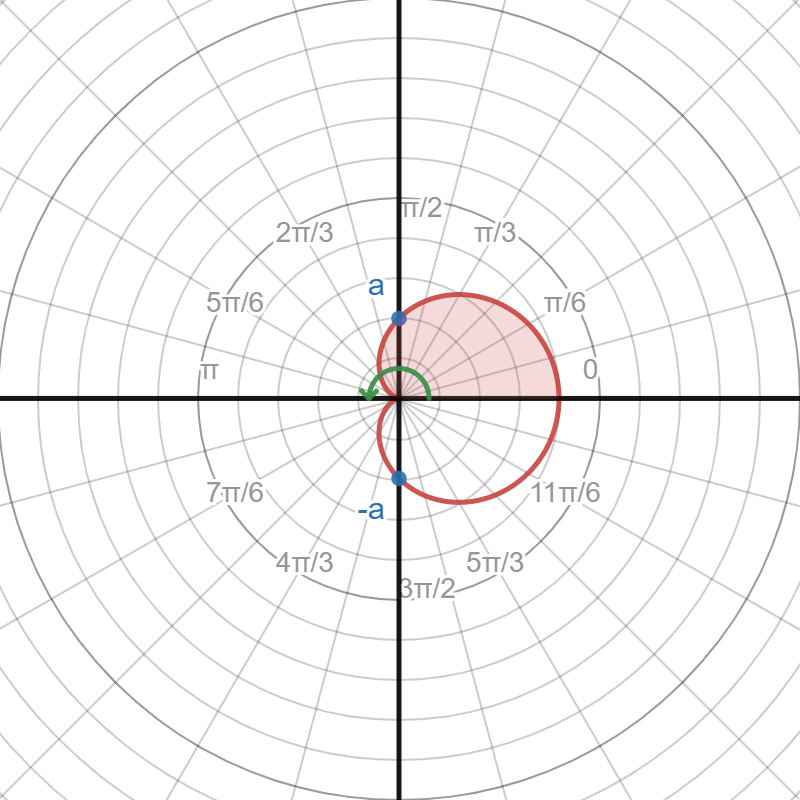
\includegraphics[width=0.6\textwidth]{1-a.png}
%\end{figure}

\large{
    We know,
    \begin{align*}
        x & = r \cos \theta \\
        y & = r \sin \theta \\
        dx \; dy & = \; \mid J \mid dr \; d\theta
    \end{align*}

Now,
\begin{align*}
    \mid J \mid
    & =
    \begin{vmatrix}
        \frac{\partial x}{\partial r} & \frac{\partial x}{\partial \theta} \\\\
        \frac{\partial y}{\partial r} & \frac{\partial y}{\partial \theta}
    \end{vmatrix}
     \\
    & =
    \begin{vmatrix}
        \cos \theta & -r \sin \theta \\
        \sin \theta & r \cos \theta
    \end{vmatrix} \\
    & = r \cos^2 (\theta) - (-r \sin^2 (\theta)) \\
    & = r \cos^2 (\theta) + r \sin^2 (\theta) \\
    & = r \{ \cos^2 (\theta) + \sin^2 (\theta) \} \\
    \mid J \mid
    & = r \\
    \therefore dx \; dy & = r \; dr \; d\theta
\end{align*}

\begin{align*}
    \iint_R xy \; dx \; dy	& = \iint_R (r \cos \theta) (r \sin \theta) \; r \; dr \; d\theta \\
                            & = \iint_R r^3 \sin \theta \cos \theta \; dr \; d\theta \\
    \iint_R y \; dx \; dy	& = \iint_R r \sin \theta \; r \; dr \; d\theta \\
                            & = \iint_R r^2 \; \sin \theta \; dr \; d\theta \\
    \therefore \frac{\iint_R xy \; dx \; dy}{\iint_R y \; dx \; dy} & = \frac{\iint_R r^3 \sin \theta \cos \theta \; dr \; d\theta}{\iint_R r^2 \; \sin \theta \; dr \; d\theta}
\end{align*}

The region 'R' is revolved around x-axis, so the axis of symmetry is the x-axis. Therefore, the center of gravity will be on the axis of symmetry (x-axis). Thus, y and z must be zero.
}

\newpage
\subsection{}%1.b

\large{

\begin{figure}[h]
    \centering
    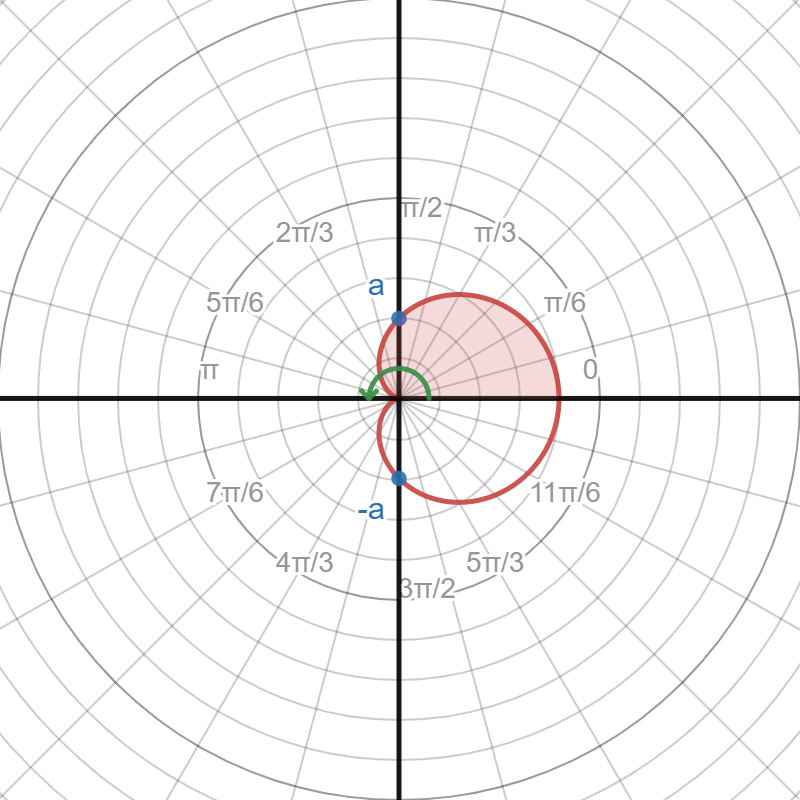
\includegraphics[width=0.6\textwidth]{1-a.png}
\end{figure}

\vspace{1cm}

Here, x-axis is the symmetry for the given shape. Using symmetry, we can find the integral for the shaded region and then multiply it by 2.
For shaded region, Range:
\begin{align*}
    0 \; \leq \; &\theta \leq \pi \\
    0 \leq r \leq & \; a(1+\cos \theta) \\
\end{align*}
\begin{align*}
\overline{X}	& = \frac{\iint_R r^3 \sin \theta \cos \theta \; dr \; d\theta}{\iint_R r^2 \; \sin \theta \; dr \; d\theta} \\
				& = \frac{\int^\pi_0 \int^{a(1+\cos \theta)}_0 r^3 \sin \theta \cos \theta \; dr \; d\theta}{\int^\pi_0 \int^{a(1+\cos \theta)}_0 r^2 \; \sin \theta \; dr \; d\theta}
\end{align*}

Considering for one side of the symmetry ($0$ to $\pi$).
\begin{align*}
    \int^\pi_0 \int^{a(1+\cos \theta)}_0 r^3 \sin \theta \cos \theta \; dr \; d\theta & = \int^\pi_0 \left[ \frac{r^4}{4} \sin \theta \cos \theta \right]^{a(1+\cos \theta)}_0 \; d\theta \\
    & = \frac{1}{4} \int^\pi_0 a^4 (1+\cos \theta)^4 \sin \theta \cos \theta \; d\theta \\
    & = \frac{a^4}{4} \int^\pi_0 (1+\cos \theta)^4 \sin \theta \cos \theta \; d\theta \\
\end{align*}

Let,
\begin{align*}											& \\
    u															& = \cos \theta \\
    \therefore du												& = -\sin (\theta) d\theta \\
    \int (1+\cos \theta)^4 \sin \theta \cos \theta \; d\theta
    & = \int (1+u)^4 u (-du) \\
    & = -\int u(1+u)^4 du \\
    Let, \quad\quad												& \\
    s															& = 1+u \\
    \therefore ds												& = du \\
    -\int u(1+u)^4 du											& = -\int (s-1)s^4 ds \\
                                                                & = \int s^4 - s^5 ds \\
                                                                & = \frac{s^5}{5} - \frac{s^6}{6} + C \\
                                                                & = \frac{(1+u)^5}{5} - \frac{(1+u)^6}{6} + C \\
    \therefore \int (1+\cos \theta)^4 \sin \theta \cos \theta \; d\theta
                                                                & = \frac{(1+\cos \theta)^5}{5} - \frac{(1+\cos \theta)^6}{6} + C \\
\end{align*}

Now,
\begin{align*}
    \frac{a^4}{4} \int^\pi_0 (1+\cos \theta)^4 \sin \theta \cos \theta \; d\theta
    & = \frac{a^4}{4} \left[ \frac{(1+\cos \theta)^5}{5} - \frac{(1+\cos \theta)^6}{6} \right]^\pi_0 \\
    & = \frac{a^4}{4} \left\{ \frac{32}{5} - \frac{32}{3} \right\} \\
    \therefore \int^\pi_0 \int^{a(1+\cos \theta)}_0 r^3 \sin \theta \cos \theta \; dr \; d\theta
    & = -\frac{16}{15} a^4
\end{align*}

Again,
\begin{align*}
    \int^\pi_0 \int^{a(1+\cos \theta)}_0 r^2 \; \sin \theta \; dr \; d\theta
    & = \int^\pi_0 \left[ \frac{r^3}{3} \sin \theta \right]^{a(1+\cos \theta)}_0 \; d\theta \\
    & = \frac{1}{3} \int^\pi_0 a^3 (1+\cos \theta)^3 \sin \theta \; d\theta \\
    & = \frac{a^3}{3} \int^\pi_0 (1+\cos \theta)^3 \sin \theta \; d\theta \\
\end{align*}

Let,
\begin{align*}
    u															& = \cos \theta \\
    \therefore du												& = -\sin (\theta) d\theta \\
    \int (1+\cos \theta)^3 \sin \theta \; d\theta
    & = \int (1+u)^3 \; (-du) \\
    & = -\int (1+u)^3 du \\
    Let, \quad\quad												& \\
    s															& = 1+u \\
    \therefore ds												& = du \\
    -\int (1+u)^3 du											& = -\int s^3 ds \\
                                                                & = -\frac{s^4}{4} + C \\
                                                                & = -\frac{(1+u)^4}{4} + C \\
    \therefore \int (1+\cos \theta)^3 \sin \theta \; d\theta	& = -\frac{(1+ \cos \theta)^4}{4} + C \\
\end{align*}

Now,
\begin{align*}
    \frac{a^3}{3} \int^\pi_0 (1+\cos \theta)^3 \sin \theta \; d\theta
    & = \frac{a^3}{3} \left[ -\frac{(1+ \cos \theta)^4}{4} \right]^\pi_0 \\
    & = \frac{a^3}{3} (-4) \\
    \therefore \int^\pi_0 \int^{a(1+\cos \theta)}_0 r^2 \; \sin \theta \; dr \; d\theta
    & = -\frac{4}{3} a^3
\end{align*}

for the entire rotation we multiply with 2.
\begin{align*}
    \overline{X}			& = \frac{\int^\pi_0 \int^{a(1+\cos \theta)}_0 r^3 \sin \theta \cos \theta \; dr \; d\theta}{\int^\pi_0 \int^{a(1+\cos \theta)}_0 r^2 \; \sin \theta \; dr \; d\theta} \times 2\\
                            & = \frac{-\dfrac{16}{15} a^4}{-\dfrac{4}{3} a^3} \times 2\\
    \therefore \overline{X}	& = \frac{8}{5} a
\end{align*}

$\therefore$ Center of gravity = $\left( \dfrac{8}{5}a,\, 0,\, 0 \right)$
}

\newpage
\subsection{}%1.c
\large{

\begin{align*}
    \text{Surface Area}	& = \iint_R f(x) \; dx \; dy \\
\end{align*}
Given,
\begin{align*}
V				& = 2 \pi \iint_R f(x) \; dx \; dy \\
				& = 2 \pi \iint_R r \sin \theta \; dx \; dy \; ; \; [\because y = f(x) = r \sin \theta]
\end{align*}

\begin{align*}
    We\;know, \quad\quad \\
    dx \; dy \; & = \; \mid J \mid \; dr \; d\theta \\
\end{align*}

Now,
\begin{align*}
    \mid J \mid
    & =
    \Large{
    \begin{vmatrix}
    \frac{\partial x}{\partial r} & \frac{\partial x}{\partial \theta} \\\\
    \frac{\partial y}{\partial r} & \frac{\partial y}{\partial \theta}
    \end{vmatrix}
    }\\
    & = 
    \begin{vmatrix}
    \cos \theta & -r \sin \theta \\
    \sin \theta & r \cos \theta
    \end{vmatrix} \\
    & = r \cos^2 (\theta) - (-r \sin^2 (\theta)) \\
    & = r \cos^2 (\theta) + r \sin^2 (\theta) \\
    & = r \{ \cos^2 (\theta) + \sin^2 (\theta) \} \\
    \mid J \mid
    & = r \\
    \therefore dx \; dy & = r \; dr \; d\theta
\end{align*}

\begin{align*}
    V				& = 2 \pi \iint_R r \sin \theta \; dx \; dy \\
                    & = 2 \pi \iint_R r \sin \theta \; r \; dr \; d\theta \\
    \therefore V	& = 2 \pi \iint_R r^2 \sin \theta \; dr \; d\theta \\
\end{align*}

}

\newpage
\subsection{}%1.d
\large{

\begin{align*}
    V &= 2\pi \int \int_R r^2\sin\theta dr d\theta\\
    &=2\pi \int_{\theta = 0}^{\theta=\pi}\int_{r=0}^{r=a(1+\cos\theta)}r^2\sin\theta drd\theta\\
    &=2\pi \int_0^\pi\Bigg[\frac{r^3}{3}\Bigg]_0^{a(1+\cos\theta)}\sin\theta d\theta\\
    &=\frac{2\pi}{3}\int_0^\pi a^3(1+\cos\theta)^3\sin\theta d\theta\\
\end{align*}

Let,
\begin{eqnarray*}
    u &=& 1+\cos{\theta}\\
    \therefore\; \sin{\theta}\;d\theta &=& -du\\
\end{eqnarray*}

\begin{center}
    \begin{tabular}{ | c | c | c | }
        \hline
        $\theta$  & 0 & $\pi$\\
        \hline
        $u$     & 2 & 0 \\
        \hline
    \end{tabular}
\end{center}


\begin{eqnarray*}
    \therefore V &=& \frac{2\pi}{3}\int_2^0a^3u^3(-du)\\
                 &=& \frac{-2\pi a^3}{3}\int_2^0u^3du\\
                 &=& \frac{-2\pi a^3}{3}\Bigg[\frac{u^4}{4}\Bigg]_2^0\\
                 &=& \frac{-2\pi a^3}{3}\Bigg[0-\frac{16}{4}\Bigg]\\ 
                 &=& \frac{8\pi a^3}{3}\\
\end{eqnarray*}

}

\newpage
\subsection{}%1.e
\large{
\begin{eqnarray*}
    L &=& \int_p^q\sqrt{1+[f'(x)]^2}dx\\
      &=& \int_p^q\sqrt{1+\Bigg(\frac{dy}{dx}\Bigg)^2}dx\\ 
      &=& \int_p^q \sqrt{\frac{dx^2+dy^2}{dx^2}}dx\\
      &=& \int_p^q \sqrt{(dx^2)\Bigg(\frac{dx^2+dy^2}{dx^2}\Bigg)}\\
      &=& \int\sqrt{dx^2+dy^2}\\
\end{eqnarray*}

Now,
\begin{eqnarray*}
    dL &=& \sqrt{dx^2+dy^2}\\
    \implies dL^2 &=& dx^2+dy^2\\
    \implies\frac{dL^2}{d\theta^2} &=& \frac{dx^2}{d\theta ^2}+\frac{dy^2}{d\theta^2}\\
    \implies dL^2 &=& \Bigg[\Bigg(\frac{dx}{d\theta}\Bigg)^2+\Bigg(\frac{dy}{d\theta}\Bigg)^2\Bigg]d\theta ^2\\
    \implies dL &=& \sqrt{\Bigg(\frac{dx}{d\theta}\Bigg)^2+\Bigg(\frac{dy}{d\theta}\Bigg)^2}d\theta\\
                &&\text{[integrating both sides]}\\
    \therefore L &=& \int_a^b \sqrt{\Bigg(\frac{dx}{d\theta}\Bigg)^2+\Bigg(\frac{dy}{d\theta}\Bigg)^2}d\theta\\
\end{eqnarray*}

\newpage
Now,

\begin{align*}
    x &= r(\theta) \cos\theta\\
    y&=r(\theta) \sin \theta\\
    \therefore \Bigg(\frac{dx}{d\theta}\Bigg)^2 &= \Bigg(-r\sin\theta+\cos\theta\frac{dr}{d\theta}\Bigg)^2\\
    \therefore \Bigg(\frac{dy}{d\theta}\Bigg)^2 &= \Bigg(r\cos\theta+\sin\theta\frac{dr}{d\theta}\Bigg)^2\\
    \therefore dL^2 &= \Bigg[\cos^2\theta\Bigg(\frac{dr}{d\theta}\Bigg)^2-2r\sin\theta \cos\theta \Bigg(\frac{dr}{d\theta}\Bigg)+r^2\sin^2\theta +\\&\hspace{2em}r^2\cos^2\theta+2r\sin\theta \cos\theta\Bigg(\frac{dr}{d\theta}\Bigg)+\sin^2\theta\Bigg(\frac{dr}{d\theta}\Bigg)^2\Bigg]d\theta^2\\
    \implies dL^2 &= \Bigg[r^2(\sin^2\theta+\cos^2\theta)+\Bigg(\frac{dr}{d\theta}\Bigg)^2(\sin^2\theta + \cos^2\theta)\Bigg]d\theta^2\\
    \implies dL^2 &= \Bigg[r^2+\Bigg(\frac{dr}{d\theta}\Bigg)^2\Bigg]d\theta^2\\
    \therefore dL &= \sqrt{r^2+\Bigg(\frac{dr}{d\theta}\Bigg)^2}d\theta\\
    &\text{[integrating both sides]}\\
    \therefore L &= \int_a^b\sqrt{r^2+\Bigg[\frac{dr}{d\theta}\Bigg]^2}d\theta\\
\end{align*}
\hspace{7cm}[proved]

}
\newpage
\subsection{}%1.f
\large{
\begin{align*}
    L &= \int_a^b\sqrt{r^2+\Bigg(\frac{dr}{d\theta}\Bigg)^2}d\theta\\
    r &= a(1+\cos\theta)\\
    &= a + a\cos\theta\\
    \therefore \frac{dr}{d\theta} &= -a\sin\theta\\
    \therefore \Bigg(\frac{dr}{d\theta}\Bigg)^2&=a^2\sin^2\theta\\
    \therefore \text{Perimeter:}\\
    &= 2\int_0^\pi \sqrt{[a^2(1+\cos\theta)^2]+a^2\sin\theta}d\theta\\
    &=2\int_0^\pi\sqrt{[a^2(1+2\cos\theta+\cos^2\theta)]+a^2\sin\theta}d\theta\\
    &= 2\int_0^\pi \sqrt{a^2(1+2\cos\theta+\cos^2\theta+\sin^2\theta)}d\theta\\
    &=2a\int_0^\pi\sqrt{2+2\cos\theta}d\theta\\ &= 2a\int_0^\pi\sqrt{2(1+\cos\theta)}d\theta\\
    &=2a\int_0^\pi\sqrt{2\Bigg[2\cos^2\Bigg(\frac{\theta}{2}\Bigg)\Bigg]}d\theta\\
    &=4a\int_0^\pi \cos\Bigg(\frac{\theta}{2}\Bigg)d\theta\\
    &=4a\Bigg[\frac{\sin(\theta/2)}{1/2}\Bigg]_0^\pi\\ &= 8a(\sin(\pi/2)-\sin0)\\
    &=8a\\
\end{align*}
}


\newpage
\section{Particle in a Cylinder}
\subsection{}%2.a
\large{
$$<\psi|\psi> = 1 $$
The probability of finding the particle outside S is 0 and the probability of finding the particle inside S is non-zero; hence the summation of all probabilities (total probability of finding the particle inside S) is 1.
}

\vspace{2cm}

\subsection{}%2.b
\large{
The cylindrical coordinate system will be a good choice to evaluate the integrals because it is easier to determine the limits for the given bounded region and equation. It is also easier to convert the equation to a simpler form ($\sqrt{x^2 + y^2} = r$) using this coordinate system.
$$<g|h> \,\,= \iiint_S g(x,y,z)^{*}h(x,y,z) \,\, dV $$
For,
$$<\psi|\psi> \,\, = \iiint_S \psi(x,y,z)^{*}\psi(x,y,z) \,\, dV $$
Since, $\psi(x,y,z)$ is real and complex conjugate of a real number is also real, we can write-
\begin{eqnarray*}
        <\psi|\psi> &=& \iiint_S (\psi(x,y,z))^2 \,\, dV\\
        &=&\iiint_S \frac{A^2}{\sqrt{x^2+y^2}} \,\, dV\\
\end{eqnarray*}

\newpage
\begin{figure}[h]
    \centering
    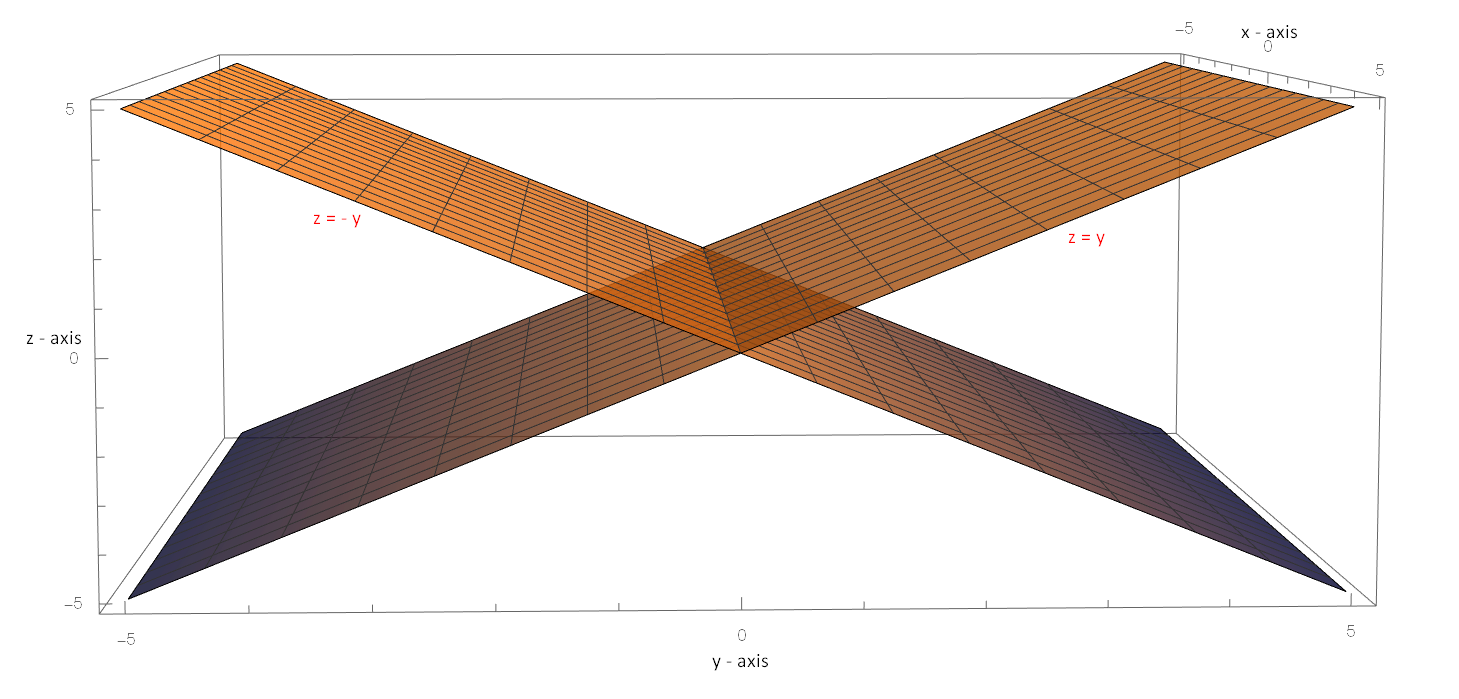
\includegraphics[width=1.0\textwidth]{2-b(i).png}
    \caption{$z=y$ and $z=-y$ planes}
\end{figure}

We know: $-y  \leq z \leq y$.\\
So in terms of cylindrical coordinate system, $ -r\sin\theta \leq z \leq r\sin\theta$.

\newpage
%\includegraphics[width=12cm,height=12cm,keepaspectratio]{desmos-graph(2.2).png}\\
\begin{figure}[h]
    \centering
    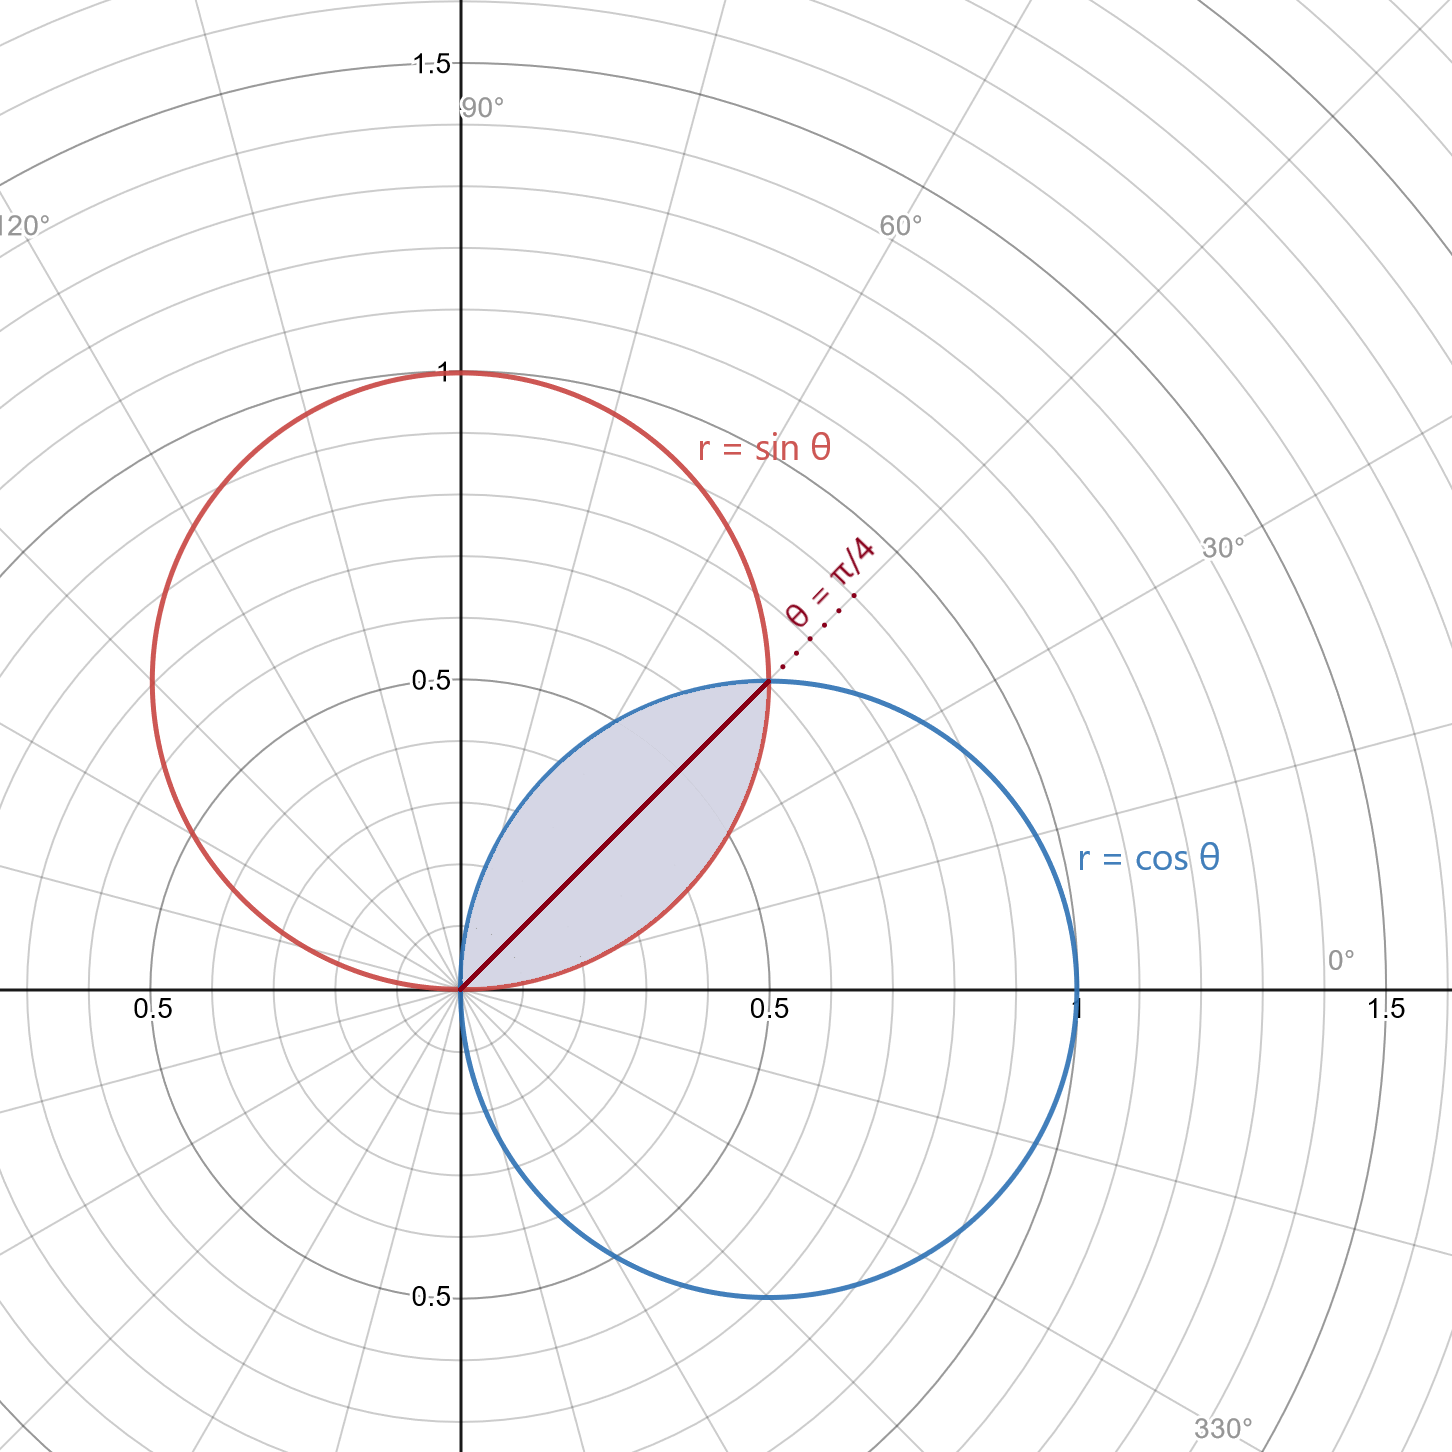
\includegraphics[width=0.7\textwidth]{2-b(ii).png}
    \caption{$xy$ plane}
\end{figure}

%$$Fig. \,xy\, plane$$\\
Using the graph above,\\
$$\sin\theta=\cos\theta$$
$$\tan\theta = 1$$
$$\theta = \frac{\pi}{4}$$
So, the limits are:\\
$$ -r\sin\theta \leq z \leq r\sin\theta$$
$$0\leq \theta\leq \frac{\pi}{4} \,\,and \,\,\frac{\pi}{4} < \theta\leq \frac{\pi}{2} $$
$$0\leq r \leq \sin\theta \,\,and \,\,0 < r \leq \cos\theta$$
Finally, putting the limits into the equation and substituting the value of $\sqrt{x^2+y^2}\, = r$.
\begin{eqnarray*}
        <\psi|\psi> &=&\iiint_S \frac{A^2}{r} \,\, dV\\
        <\psi|\psi>&=& \int_{0}^{\frac{\pi}{4}}\int_{0}^{\sin\theta}\int_{-r\sin\theta}^{r\sin\theta} \frac{A^2}{r} \,\, dV + \int_{\frac{\pi}{4}}^{\frac{\pi}{2}}\int_{0}^{\cos\theta}\int_{-r\sin\theta}^{r\sin\theta} \frac{A^2}{r} \,\, dV  \\
\end{eqnarray*}
}

\subsection{}%2.c

\large{

\begin{eqnarray*}
        dV  &=&|\frac{\partial(x,y,z)}{\partial(z,r,\theta)}|\, dz\,dr\,d\theta\\\\\\
        &=&\begin{vmatrix} \frac{\partial x}{\partial z} & \frac{\partial x}{\partial r} & \frac{\partial x}{\partial \theta} \\\\ \frac{\partial y}{\partial z} & \frac{\partial y}{\partial r} & \frac{\partial y}{\partial \theta} \\\\ \frac{\partial z}{\partial z} & \frac{\partial z}{\partial r} & \frac{\partial z}{\partial \theta} \end{vmatrix} dz\,dr\,d\theta \\\\\\
        &=&\begin{vmatrix} 0 &\cos\,\theta &  -r\sin\,\theta  \\ 0 & \sin\,\theta & r\cos\,\theta  \\ 1 & 0 & 0 \end{vmatrix} dz\,dr\,d\theta \\
        &=& (r\cdot \cos^2 \theta + r \cdot \sin^2 \theta) \,dz\,dr\,d\theta\\
        &=& r\cdot (\cos^2 \theta + \sin^2 \theta) \,dz\,dr\,d\theta\\
        &=& r\,\,dz\,dr\,d\theta\\
\end{eqnarray*}
}
\pagebreak
\subsection{}%2.d

\large{
We know, $<\psi|\psi>\,=1$. \\
So we can write,
\begin{eqnarray*}
        <\psi|\psi> \,= \int_{0}^{\frac{\pi}{4}}\int_{0}^{\sin\theta}\int_{-r\sin\theta}^{r\sin\theta} \frac{A^2}{r} \,\, dV + \int_{\frac{\pi}{4}}^{\frac{\pi}{2}}\int_{0}^{\cos\theta}\int_{-r\sin\theta}^{r\sin\theta} \frac{A^2}{r} \,\, dV  = 1\\
\end{eqnarray*}
Now, substituting the value of dV using the Jacobian determinant and solving:
\begin{eqnarray*}
        <\psi|\psi> \,&=& \int_{0}^{\frac{\pi}{4}}\int_{0}^{\sin\theta}\int_{-r\sin\theta}^{r\sin\theta} \frac{A^2}{r} \,\, \cdot r\,\,dz\,dr\,d\theta + \int_{\frac{\pi}{4}}^{\frac{\pi}{2}}\int_{0}^{\cos\theta}\int_{-r\sin\theta}^{r\sin\theta} \frac{A^2}{r} \,\, \cdot r\,\,dz\,dr\,d\theta = 1\\
        &=& \int_{0}^{\frac{\pi}{4}} \int_{0}^{\sin\theta} \int_{-r\sin\theta}^{r\sin\theta} A^2 \,\,dz\,dr\,d\theta + \int_{\frac{\pi}{4}}^{\frac{\pi}{2}}\int_{0}^{\cos\theta}\int_{-r\sin\theta}^{r\sin\theta} A^2 \,\,dz\,dr\,d\theta = 1\\
        &=& \int_{0}^{\frac{\pi}{4}} \int_{0}^{\sin\theta} [A^2 z]_{-r\sin\theta}^{r\sin\theta} \,\,dr\,d\theta + \int_{\frac{\pi}{4}}^{\frac{\pi}{2}}\int_{0}^{\cos\theta}  [A^2 z]_{-r\sin\theta}^{r\sin\theta} \,\,dr\,d\theta = 1\\
        &=& \int_{0}^{\frac{\pi}{4}} \int_{0}^{\sin\theta} 2A^2 r\sin\,\theta \,\,dr\,d\theta + \int_{\frac{\pi}{4}}^{\frac{\pi}{2}}\int_{0}^{\cos\theta}  2A^2 r\sin\,\theta  \,\,dr\,d\theta = 1\\
        &=& \int_{0}^{\frac{\pi}{4}} [A^2 r^2\sin\,\theta]_{0}^{\sin\theta}  \,\,d\theta + \int_{\frac{\pi}{4}}^{\frac{\pi}{2}}  [A^2 r^2\sin\,\theta]_{0}^{\cos\theta}  \,\,d\theta = 1\\
        &=& \int_{0}^{\frac{\pi}{4}} A^2 \sin^3 \theta  \,\,d\theta + \int_{\frac{\pi}{4}}^{\frac{\pi}{2}}  A^2 \cos^2\theta \sin\,\theta  \,\,d\theta = 1\\
        &=& A^2  \int_{0}^{\frac{\pi}{4}} \sin^3 \theta  \,\,d\theta + A^2 \int_{\frac{\pi}{4}}^{\frac{\pi}{2}} \cos^2\theta \sin\,\theta  \,\,d\theta = 1\\
\end{eqnarray*}
First,
$$\int \sin^3 \theta  \,\,d\theta\, =\int (1- \cos^2\theta)\sin\,\theta  \,\,d\theta $$
Let $u=\cos\,\theta$ and $\frac{du}{d\theta} = -\sin\,\theta$.
$$\int -1 + u^2  \,\,du = [-u + \frac{u^3}{3}]=[-\cos\,\theta + \frac{\cos^3\theta}{3}]$$
Likewise for,
$$\int \cos^2\theta \sin\,\theta  \,\,d\theta$$
Let $u=\cos\,\theta$ and $\frac{du}{d\theta} = -\sin\,\theta$.
$$\int -u^2  \,\,du = [-\frac{u^3}{3}] = [-\frac{\cos^3\theta}{3}]$$

So putting the limits into these integrals,
\begin{eqnarray*}
 &&A^2 [-\cos\,\theta + \frac{\cos^3\theta}{3}]_{0}^{\frac{\pi}{4}} + A^2[-\frac{\cos^3\theta}{3}]_{\frac{\pi}{4}}^{\frac{\pi}{2}} = 1\\
 &&A^2[-\frac{\sqrt{2}}{2}+\frac{\sqrt{2}}{12}-(-1+\frac{1}{3})] + A^2[0-(-\frac{\sqrt{2}}{12})] = 1\\
 &&\frac{2-\sqrt{2}}{3} A^2 = 1\\
 &&A^2 = \frac{6 + 3\sqrt{2}}{2}\\
 && A = (\frac{6 + 3\sqrt{2}}{2})^\frac{1}{2}
\end{eqnarray*}
}

\subsection{}%2.e
\large{

We know,
$$<\psi|\hat{r}\psi> \, = \iiint_S \psi(x,y,z)^*\;\hat{r}\psi(x,y,z) \,\, dV\\ $$
Since, $\hat{r}\psi = r\psi$,\\
\begin{eqnarray*}
        <\psi|\hat{r}\psi> \,&=& \iiint_S (\psi(x,y,z))^2 \cdot r \,\, dV\\
        &=&\iiint_S \frac{A^2}{r} \cdot r \,\, dV\\
        &=&\int_{0}^{\frac{\pi}{4}}\int_{0}^{\sin\theta}\int_{-r\sin\theta}^{r\sin\theta} A^2 \,\, \cdot r\,\,dz\,dr\,d\theta + \int_{\frac{\pi}{4}}^{\frac{\pi}{2}}\int_{0}^{\cos\theta}\int_{-r\sin\theta}^{r\sin\theta} A^2 \,\, \cdot r\,\,dz\,dr\,d\theta \\
        &=& \int_{0}^{\frac{\pi}{4}} \int_{0}^{\sin\theta} [A^2 rz]_{-r\sin\theta}^{r\sin\theta} \,\,dr\,d\theta + \int_{\frac{\pi}{4}}^{\frac{\pi}{2}}\int_{0}^{\cos\theta}  [A^2r z]_{-r\sin\theta}^{r\sin\theta} \,\,dr\,d\theta\\
        &=& \int_{0}^{\frac{\pi}{4}} \int_{0}^{\sin\theta} 2A^2 r^2 \sin\,\theta \,\,dr\,d\theta + \int_{\frac{\pi}{4}}^{\frac{\pi}{2}}\int_{0}^{\cos\theta}  2A^2 r^2 \sin\,\theta  \,\,dr\,d\theta \\
        &=& \int_{0}^{\frac{\pi}{4}} [\frac{2A^2 r^3\sin\,\theta}{3}]_{0}^{\sin\theta}  \,\,d\theta + \int_{\frac{\pi}{4}}^{\frac{\pi}{2}}  [\frac{2A^2 r^3\sin\,\theta}{3}]_{0}^{\cos\theta}  \,\,d\theta \\
        &=& \int_{0}^{\frac{\pi}{4}} \frac{2A^2 \sin^4\theta}{3}  \,\,d\theta + \int_{\frac{\pi}{4}}^{\frac{\pi}{2}} \frac{ 2A^2 \cos^3\theta \sin\,\theta }{3}  \,\,d\theta \\
        &=& \frac{2A^2 }{3} \int_{0}^{\frac{\pi}{4}} \sin^4\theta  \,\,d\theta + \frac{ 2A^2 }{3}\int_{\frac{\pi}{4}}^{\frac{\pi}{2}} \cos^3\theta \sin\,\theta  \,\,d\theta \\
\end{eqnarray*}
For,
$$\int_{0}^{\frac{\pi}{4}} \sin^4\theta  \,\,d\theta  = \int_{0}^{\frac{\pi}{4}} \sin^3\theta \sin\,\theta  \,\,d\theta $$
Applying integration by parts such that, $f(x) = \sin^3 \theta$ and $g'(x) = \sin\,\theta$ :
\begin{eqnarray*}
       \int_{0}^{\frac{\pi}{4}} \sin^3\theta \sin\,\theta  \,\,d\theta &=& [-\sin^3\theta     \cos \,\theta - \int -3\sin^2\cos^2\theta \,\, d\theta]_{0}^{\frac{\pi}{4}}\\
\end{eqnarray*}
Using trigonometric identities we know:\\
$$3\;\sin^2\theta\;\cos^2\theta =3\left(\frac{\sin\, 2\theta}{2}\right)^2= \frac{3}{8}(1-\cos\, 4\theta)$$\\
So, substituting this value:
\begin{eqnarray*}
        \int_{0}^{\frac{\pi}{4}} \sin^3\theta \sin\,\theta  \,\,d\theta &=& [-\sin^3\theta \cos \,\theta -  \frac{3}{8}\int(1-\cos\, 4\theta)]_{0}^{\frac{\pi}{4}}\\
        &=&[-\sin^3\theta \cos \,\theta -  \frac{3}{8}(\theta -\frac{\sin\,4\theta}{4})]_{0}^{\frac{\pi}{4}}\\
        &=&\frac{3\pi-8}{32}
\end{eqnarray*}
Now for,
$$\int_{\frac{\pi}{4}}^{\frac{\pi}{2}} \cos^3\theta \sin\,\theta  \,\,d\theta$$
Let $u=\cos\,\theta$ and $\frac{du}{d\theta} = -\sin\,\theta$.
\begin{eqnarray*}
        \int_{\frac{\pi}{4}}^{\frac{\pi}{2}} \cos^3\theta \sin\,\theta  \,\,d\theta &=&  \int -u^3 du\\
        &=&[-\frac{u^4}{4}]\\
        &=&[\frac{-\cos^4\theta}{4}]_{\frac{\pi}{4}}^{\frac{\pi}{2}} \\
        &=&\frac{1}{16}
\end{eqnarray*}
Putting these values into the original equation of $<\psi|\hat{r}\psi>$
\begin{eqnarray*}
    <\psi|\hat{r}\psi> \,&=&  \frac{2A^2 }{3}\cdot \frac{3\pi-8}{32} + \frac{ 2A^2 }{3}\cdot \frac{1}{16} \\
    &=&\frac{3\pi-8}{48}A^2+\frac{1}{24}A^2\\
    &=& \frac{3\pi-6}{48} A^2
\end{eqnarray*}
Finally putting the value of $A^2 = \frac{6+3\sqrt{2}}{2}$ (known from 2c)
\begin{eqnarray*}
    <\psi|\hat{r}\psi> &=&\frac{3\pi-6}{48}\cdot\frac{6+3\sqrt{2}}{2}\\
    &=&\frac{18\pi + 9\pi\sqrt{2}-36-18\sqrt{2}}{96}\\
\end{eqnarray*}
}


\subsection{}%2.f
\large{
If $\hat{A}(kf) = k\hat{A}f$ and $\hat{r}\psi = r\psi$, \\
Then, \\
$$\hat{r}^2\psi = \hat{r}(\hat{r}\psi) = \hat{r}(r\psi) = r^2\psi$$
}

\vspace{2cm}

\subsection{}%2.g
\large{
\begin{eqnarray*}
        <\psi|\hat{r}^2\psi> &=&  \iiint_S \psi(x,y,z)^*\;\hat{r}^2\psi(x,y,z) \,\, dV\\
        &=& \iiint_S\frac{A^2}{r} \cdot r^2 \,\, dV\\
        &=&\int_{0}^{\frac{\pi}{4}}\int_{0}^{\sin\theta}\int_{-r\sin\theta}^{r\sin\theta} A^2 \,\, \cdot r^2\,\,dz\,dr\,d\theta + \int_{\frac{\pi}{4}}^{\frac{\pi}{2}}\int_{0}^{\cos\theta}\int_{-r\sin\theta}^{r\sin\theta} A^2 \,\, \cdot r^2\,\,dz\,dr\,d\theta \\
        &=& \int_{0}^{\frac{\pi}{4}} \int_{0}^{\sin\theta} [A^2 r^2z]_{-r\sin\theta}^{r\sin\theta} \,\,dr\,d\theta + \int_{\frac{\pi}{4}}^{\frac{\pi}{2}}\int_{0}^{\cos\theta}  [A^2r^2 z]_{-r\sin\theta}^{r\sin\theta} \,\,dr\,d\theta\\
        &=& \int_{0}^{\frac{\pi}{4}} \int_{0}^{\sin\theta} 2A^2 r^3 \sin\,\theta \,\,dr\,d\theta + \int_{\frac{\pi}{4}}^{\frac{\pi}{2}}\int_{0}^{\cos\theta}  2A^2 r^3 \sin\,\theta  \,\,dr\,d\theta \\
        &=& \int_{0}^{\frac{\pi}{4}} [\frac{A^2 r^4\sin\,\theta}{2}]_{0}^{\sin\theta}  \,\,d\theta + \int_{\frac{\pi}{4}}^{\frac{\pi}{2}}  [\frac{A^2 r^4\sin\,\theta}{2}]_{0}^{\cos\theta}  \,\,d\theta \\
        &=& \int_{0}^{\frac{\pi}{4}} \frac{A^2 \sin^4\theta \sin\,\theta}{2}  \,\,d\theta + \int_{\frac{\pi}{4}}^{\frac{\pi}{2}} \frac{ A^2 \cos^4\theta \sin\,\theta }{2}  \,\,d\theta \\
        &=& \frac{A^2 }{2} \int_{0}^{\frac{\pi}{4}}  \sin^4\theta \sin\,\theta \,\,d\theta + \frac{ A^2 }{2}\int_{\frac{\pi}{4}}^{\frac{\pi}{2}}  \cos^4\theta \sin\,\theta  \,\,d\theta \\
        &=& \frac{A^2 }{2} \int_{0}^{\frac{\pi}{4}}  (1-\cos^2\theta)^2\theta \sin\,\theta \,\,d\theta + \frac{ A^2 }{2}\int_{\frac{\pi}{4}}^{\frac{\pi}{2}}  \cos^4\theta \sin\,\theta  \,\,d\theta \\
\end{eqnarray*}
Let $u=\cos\,\theta$ and $\frac{du}{d\theta} = -\sin\,\theta$.
\begin{eqnarray*}
        <\psi|\hat{r}^2\psi> &=&\frac{A^2 }{2} \int -1 + 2u^2 - u^4 \,\, du +\frac{A^2 }{2} \int -u^4 \,\,du\\
        &=&\frac{A^2 }{2} [-u + \frac{2u^3}{3} - \frac{u^5}{5}] +\frac{A^2 }{2} [\frac{-u^5}{5}] \\
        &=&\frac{A^2 }{2} [-\cos\,\theta + \frac{2\cos^3\theta}{3} - \frac{\cos^5\theta}{5}]_{0}^{\frac{\pi}{4}} +\frac{A^2 }{2} [\frac{-\cos^5\theta}{5}]_{\frac{\pi}{4}}^{\frac{\pi}{2}} \\
        &=&\frac{A^2 }{2} (\frac{32\sqrt{2}-43}{60\sqrt{2}}) +\frac{A^2 }{2} (\frac{1}{20\sqrt{2}}) \\
        &=& A^2 (\frac{32\sqrt{2}-43}{120\sqrt{2}}) +A^2 (\frac{1}{40\sqrt{2}}) \\
        &=& (\frac{4\sqrt{2}-5}{15\sqrt{2}})A^2 \\
\end{eqnarray*}
Finally substituting the value of $A^2 = \frac{6+3\sqrt{2}}{2}$ (known from 2c),

\begin{eqnarray*}
        <\psi|\hat{r}^2\psi> &=& \frac{4\sqrt{2}-5}{15\sqrt{2}} \cdot \frac{6+3\sqrt{2}}{2}\\
        &=&\frac{3-\sqrt{2}}{10}
\end{eqnarray*}
}

\vspace{2cm}
\subsection{}%2.h
{\large
\begin{eqnarray*}
    \sigma_r^2 &=&<\psi|\hat{r}^2\psi> - <\psi|\hat{r}\psi> ^2\\
    \sigma_r^2 &=&\frac{3-\sqrt{2}}{10} - (\frac{18\pi + 9\pi\sqrt{2} -36 - 18 \sqrt{2}}{96})^2\\
    \sigma_r^2 &=& 0.0250587\\
    \sigma_r &=& 0.1583\\
\end{eqnarray*}
}



\newpage
\section{Rotating Tube}

\subsection{}%3.a
\setcounter{equation}{0}
\begin{figure}[h]
    \centering
    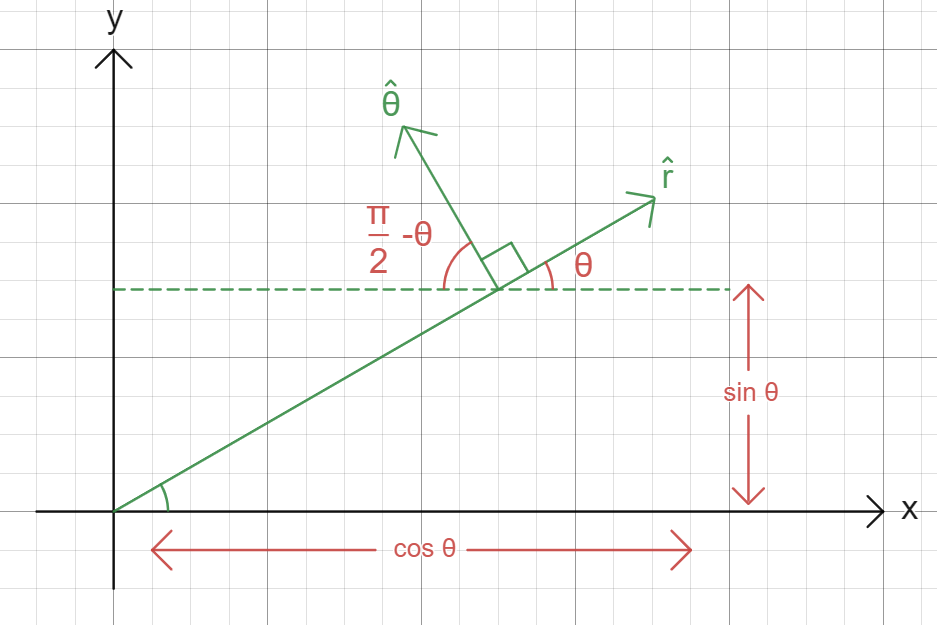
\includegraphics[width=0.7\textwidth]{3-a.PNG}
\end{figure}


\large{
    \begin{eqnarray*}
        \hat{r} &=& x\hat{i} + y\hat{j}\\
                &=& r\cos{\theta}\;\hat{i} + r\sin{\theta}\;\hat{j}\\
                &=& r(\cos{\theta}\;\hat{i} + \sin{\theta}\;\hat{j})
    \end{eqnarray*}
    Also we know,
    \begin{eqnarray*}
        \vec{r} &=& r\;\hat{r}\hspace{2cm}\text{[where $\hat{r}$ is the unit vector]}\\
        or,\; r\;\hat{r} &=& r(\cos{\theta}\;\hat{i} + \sin{\theta}\;\hat{j})\\
        \therefore\;\hat{r} &=& \cos{\theta}\;\hat{i} + \sin{\theta}\;\hat{j}
    \end{eqnarray*}
    From the figure,
    \begin{eqnarray*}
        \hat{\theta} &=& -\cos{\left(\frac{\pi}{2} - \theta\right)}\;\hat{i} + \sin{\left(\frac{\pi}{2} - \theta\right)}\;\hat{j}\\
                     &=& -\sin{\theta}\;\hat{i} + \cos{\theta}\;\hat{j}
    \end{eqnarray*}
    According to question,
    \begin{align}
        v &= \frac{dr}{dt}\;\hat{r} + r\;\frac{d\theta}{dt}\;\hat{\theta}\notag\\
        or,\; v&= r'(t)\;\hat{r} + r\;\theta'(t)\;\hat{\theta}\notag\\
        or,\; \frac{dv}{dt} &= \frac{d}{dt}\left(r'(t)\;\hat{r} + r\;\theta'(t)\;\hat{\theta}\right)\notag\\
        or,\; f_r &= r''(t)\;\hat{r} + r'\;\frac{d\hat{r}}{dt} + r'\theta'(t)\;\hat{\theta} + r\;\theta''(t)\;\hat{\theta}+r\;\theta'(t) \;\frac{d\hat{\theta}}{dt}
    \end{align}

    now,
    \begin{eqnarray*}
        \frac{d\hat{r}}{dt} &=& \frac{d}{dt}\left(\cos{\theta}\;\hat{i} + \sin{\theta}\;\hat{j}\right)\\
                            &=& \theta'(t)\left(-\sin{\theta}\;\hat{i} + \cos{\theta}\;\hat{j}\right)\\
                            &=& \theta'(t)\;\hat{\theta}
    \end{eqnarray*}
    \begin{eqnarray*}
        \frac{d\hat{\theta}}{dt} &=& \frac{d}{dt}\left(-\sin{\theta}\;\hat{i} + \cos{\theta}\hat{j}\right)\\
                                 &=& -\theta'(t)\cos{\theta}\;\hat{i} - \theta'(t)\sin{\theta}\;\hat{j}\\
                                 &=& -\theta'(t)\;[\cos{\theta} + \sin{\theta}]\\
                                 &=& -\theta'(t)\;\hat{r}\\
    \end{eqnarray*}

    if we substitute in (3.1) we get,

    \begin{eqnarray*}
        f_r &=& r''(t)\;\hat{r} + r'\;\frac{d\hat{r}}{dt} + r'\theta'(t)\;\hat{\theta} + r\;\theta''(t)\;\hat{\theta}+r\;\theta'(t) \;\frac{d\hat{\theta}}{dt}\\
        f_r &=& r''(t)\;\hat{r} + r'\;\theta'(t)\;\hat{\theta} + r'(t)\;\theta'(t)\;\hat{\theta} + r\;\theta''(t)\;\hat{\theta}+r\;\theta'(t)\left[-\theta'(t)\;\hat{r}\right]\\
    \end{eqnarray*}

    considering $r$ components,
    \begin{eqnarray*}
        f_r &=& r''(t) + r\;\theta'(t)\times[-\theta'(t)]\\
            &=& r''(t) - r\left\{(\theta'(t)\right\}^2\\
    \end{eqnarray*}
    $$\therefore f_r = \frac{d\;r^2}{dt} - r\left(\frac{d\theta}{dt}\right)^2$$
    \hspace{10cm}[proved]


}


\newpage

\subsection{}%3.b
\large{
If we consider the particles $F$ or Force's components. There will be two components one is $mg\cos\theta$ and the other one is $mg\sin\theta$. The only Force is active during rotation is $mg\sin\theta$. Because the force is directly proportional to sine of the angular displacement. So we get,
$$F = -mg\sin{\omega t}$$
We also know, $F=ma$ or $F=m\cdot f_r$ . If we substitute,
\begin{eqnarray*}
    m\cdot f_r &=& -mg\sin{\omega t}\\
    \bcancel{m}\cdot f_r &=& -\bcancel{m}\;g\sin{\omega t}\\
    f_r &=& -g\sin{\omega t}\\
    \frac{d\;r^2}{dt} - r\;\left(\frac{d\theta}{dt}\right)^2 &=& -g\sin{\omega t}\hspace{2cm}\text{[from (a)]}\\
    \frac{d\;r^2}{dt} - r\omega^2 &=& -g\sin{\omega t} \hspace{2cm}\left[\because \omega = \frac{d\theta}{dt}\;\right]
\end{eqnarray*}
}
\hspace{8cm}[showed]



\newpage
\subsection{}%3.c
\large{
Given,
\begin{equation*}
    \frac{d^2 r}{dt^2}-r\omega^{2} = -g\sin{\omega t}
\end{equation*}

\vspace{1cm}

\begin{minipage}[t]{0.4\linewidth}
    \underline{\bfseries{C.F:}}
    $$r'' - r\omega^{2} = 0$$
    let,
    \begin{eqnarray*}
        r &=& e^{kt}\\
        r' &=& k\;e^{kt}\\
        r'' &=& k^2\;e^{kt}
    \end{eqnarray*}
    now,
    \begin{eqnarray*}
        k^2\;e^{kt} - e^{kt}\omega^2 &=& 0\\
        or,\;e^{kt} (k^2 - \omega^2) &=& 0\\
        or,\;k^2 - \omega^2 &=& 0\\
        \therefore\;k &=& \pm\;\omega
    \end{eqnarray*}
    $$C.F = C_1\;e^{\omega t} + C_2\;e^{-\omega t}$$
\end{minipage}\hfill
\begin{minipage}[t]{0.4\linewidth}
    \underline{\bfseries{P.I:}}\\
    we can write the equation as,
    $$(D^2 - \omega^2)r = -g\sin{\omega t}$$
    \begin{eqnarray*}
        \text{P.I} &=& \frac{1}{D^2 - \omega^2} \times (-g\sin{\omega t})\\
                   &=& -g\left[\frac{1}{D^2 - \omega^2}\times\sin{\omega t}\right]\\
                   &=& -g\left[\frac{1}{-\omega^2 -\omega^2}\times \sin{\omega t}\right]\\
                   &&\text{[substituting $-\omega^2$ instead of $D^2$]}\\
                   &=& -g\times\frac{\sin{\omega t}}{-2\;\omega^2}\\
                   &=& \frac{g\sin{\omega t}}{2\;\omega^2}\\
                   &=& \frac{g}{2\;\omega^2}\;\sin{\omega t}
    \end{eqnarray*}
\end{minipage}
\vspace{2cm}
\begin{eqnarray*}
    \therefore r(t) &=& C.F + P.I\\
                    &=& C_1\;e^{\omega t} + C_2\;e^{-\omega t} + \frac{g}{2\;\omega^2}\;\sin{\omega t}
\end{eqnarray*}
}
\newpage
\subsection{}%3.d
\large{
    From (c) we got,
    $$r(t) = C_1\;e^{\omega t} + C_2\;e^{-\omega t} + \frac{g}{2\;\omega^2}\;\sin{\omega t}$$

    From hyperbolic trigonometric function we know that,
    \begin{eqnarray*}
        \cosh{(a)} + \sinh{(a)} &=& e^a\\
        \cosh{(a)} - \sinh{(a)} &=& e^{-a}
    \end{eqnarray*}
    Now,

    \begin{eqnarray*}
        r(t) &=& C_1\;\{\cosh{\omega t} + \sinh{\omega t}\} + C_2\{\cosh{\omega t} - \sinh{\omega t}\} + \frac{g}{2\;\omega^2}\;\sin{\omega t}\\
             &=& C_1\;\cosh{\omega t} + C_1\;\sinh{\omega t} + C_2\;\cosh{\omega t} - C_2\;\sinh{\omega t} + \frac{g}{2\;\omega^2}\;\sin{\omega t}\\
             &=& (C_1+C_2) \cosh{\omega t} + (C_1-C_2)\sinh{\omega t} + \frac{g}{2\;\omega^2}\;\sin{\omega t}\\
    \end{eqnarray*}

    let,
    \begin{eqnarray*}
        C_1 + C_2 &=& L\\
        C_1 - C_2 &=& M
    \end{eqnarray*}

    $$\therefore r(t) = L\;\cosh{\omega t} + M\;\sinh{\omega t} + \frac{g}{2\;\omega^2}\;\sin{\omega t}$$
}

\newpage
\subsection{}%3.e
\large{
    From the question we got that when $t=0$ radius was $a$.\\
    So,
    \begin{eqnarray*}
        r(t) &=& L\;\cosh{\omega t} + M\;\sinh{\omega t} + \frac{g}{2\;\omega^2}\;\sin{\omega t}\\
        or,\; a &=& L\;\cosh{(\omega\times 0)} + M\;\sinh{(\omega\times 0)} + \frac{g}{2\;\omega^2}\;\sin{(\omega \times 0)}\\
        or,\; a &=& L + 0 + 0\hspace{2cm}
        \left[
            \begin{tabular}{ll}
                $\because\; \cosh{(0)} = 1$\\
                $\;\;\;\;\; \sinh{(0)} = 0$\\
                $\;\;\;\;\; \sin{(0)} = 0$\\
            \end{tabular}
        \right]\\
        \therefore L &=& a
    \end{eqnarray*}

    after differentiating,
    \begin{eqnarray*}
        r(t) &=& L\;\cosh{\omega t} + M\;\sinh{\omega t} + \frac{g}{2\;\omega^2}\;\sin{\omega t}\\
        or,\;\frac{dr}{dt} &=& \frac{d}{dt}\left[a\;\cosh{\omega t} + M\;\sinh{\omega t} + \frac{g}{2\;\omega^2}\;\sin{\omega t}\right]\\
        or,\; v &=& a\;\omega\;\sinh{\omega t} + M\;\omega\;\cosh{\omega t} + \frac{g}{2\;\omega}\;\cos{\omega t}\\
    \end{eqnarray*}
    when $t=0$,
    \begin{eqnarray*}
        v &=& 0 + M\;\omega + \frac{g}{2\;\omega}\\
        or,\; M\;\omega &=& v-\frac{g}{2\;\omega}\\
        or,\; M\;\omega &=& \frac{2\cdot \omega \cdot v - g}{2\;\omega}\\
        or,\; M &=& \frac{2\cdot \omega \cdot v - g}{2\;\omega^2}\\
        \therefore\; M &=& \frac{v}{\omega} - \frac{g}{2\;\omega^2}
    \end{eqnarray*}
    So,
    $$r(t) = a\cosh{\omega t}+\left(\frac{v}{\omega} - \frac{g}{2\;\omega^2}\right)\sinh{\omega t} + \frac{g}{2\;\omega^2}\;\sin{\omega t}$$
    \hspace{12cm}[showed]

}


\newpage
\section{Charged Quantam Particles}
\subsection{}%4.a

\large{
In equation (15),\\
\begin{align*}
    \psi(r,\theta,\phi) &= F(r)G(\theta,\phi)\\
    \implies \frac{\partial \psi}{\partial r} (r,\theta,\phi) &= G(\theta, \phi)\frac{d}{dr}(F(r))\\
    \implies \frac{\partial \psi}{\partial \theta} (r,\theta,\phi) &= F(r)\frac{\partial}{\partial\theta}(G(\theta, \phi))\\
    \implies \frac{\partial^2 \psi}{\partial \phi^2} (r,\theta,\phi) &= F(r)\frac{\partial^2}{\partial\phi^2}(G(\theta, \phi))\\
\end{align*}
In equation (14),\\
\begin{align*}
    -\frac{\hbar^2}{2\mu}\Big[\frac{1}{r^2}\frac{\partial}{\partial r}\Big(r^2\frac{\partial \psi}{\partial r}\Big)+\frac{1}{r^2\sin(\theta)}\frac{\partial}{\partial \theta}\Big(\sin(\theta)\frac{\partial \psi}{\partial \theta}\Big)+\frac{1}{r^2\sin^2(\theta)}\Big(\frac{\partial^2\psi}{\partial \phi^2}\Big)\Big]-\frac{Q}{4\pi \epsilon_0r}\psi &= E\psi:\\
\end{align*}
\begin{align*}
    \psi &= FG,\\
    \frac{\partial \psi}{\partial r} &= G\frac{dF}{dr},\\
    \frac{\partial \psi}{\partial \theta} &= F\frac{\partial G}{\partial \theta}\\
    \frac{\partial^2 \psi}{\partial \phi^2} &= F\frac{\partial^2G}{\partial\phi^2}\\
    \frac{\partial}{\partial r}\Big(r^2\frac{\partial \psi}{\partial r}\Big) &= \frac{\partial}{\partial r}\Big(r^2G\frac{dF}{dr}\Big)\\
    &= G\frac{d}{dr}\Big(r^2\frac{dF}{dr}\Big)\\
    \frac{\partial}{\partial \theta}\Big(\sin(\theta)\frac{\partial \psi}{\partial \theta}\Big) &= \frac{\partial}{\partial \theta}\Big(\sin(\theta)F\frac{\partial G}{\partial \theta}\Big)\\
    &= F\frac{\partial}{\partial \theta}\Big(\sin(\theta)\frac{\partial G}{\partial \theta}\Big)\\
\end{align*}
$\therefore$ equation (14) can be written as,
\begin{align*}
    -\frac{\hbar^2}{2\mu}\Big[\frac{G}{r^2}\frac{d}{dr}\Big(r^2\frac{dF}{d r}\Big)+\frac{F}{r^2\sin(\theta)}\frac{\partial}{\partial \theta}\Big(\sin(\theta)\frac{\partial G}{\partial \theta}\Big)+\frac{F}{r^2\sin^2(\theta)}\Big(\frac{\partial^2G}{\partial \phi^2}\Big)\Big]-\frac{Q}{4\pi \epsilon_0r}FG &= EFG\\
\end{align*}
\hspace{15cm}[shown]
}

\vspace{4cm}

\subsection{}%4.b

\large{
    In equation (16),
\begin{align*}
    &-\frac{\hbar^2}{2\mu}\Big[\frac{G}{r^2}\frac{d}{dr}\Big(r^2\frac{dF}{d r}\Big)+\frac{F}{r^2\sin(\theta)}\frac{\partial}{\partial \theta}\Big(\sin(\theta)\frac{\partial G}{\partial \theta}\Big)+\frac{F}{r^2\sin^2(\theta)}\Big(\frac{\partial^2G}{\partial \phi^2}\Big)\Big]-\frac{Q}{4\pi \epsilon_0r}FG = EFG\\
    &\implies \frac{\hbar^2}{2\mu}\Big[\frac{G}{r^2}\frac{d}{dr}\Big(r^2\frac{dF}{d r}\Big)+\frac{F}{r^2\sin(\theta)}\frac{\partial}{\partial \theta}\Big(\sin(\theta)\frac{\partial G}{\partial \theta}\Big)+\frac{F}{r^2\sin^2(\theta)}\Big(\frac{\partial^2G}{\partial \phi^2}\Big)\Big]+\frac{Q}{4\pi \epsilon_0r}FG + EFG = 0\\
    &\hspace{11cm}\text{[Multiplying both sides by $\frac{2\mu r^2}{FG\hbar^2}$]}\\
    &\implies \frac{r^2}{FG}\Big[\frac{G}{r^2}\frac{d}{dr}\Big(r^2\frac{dF}{dr}\Big)+ \frac{F}{r^2\sin(\theta)}\frac{\partial}{\partial \theta} \Big(\sin(\theta)\frac{\partial G}{\partial \theta}\Big) + \frac{F}{r^2\sin^2(\theta)}\Big(\frac{\partial^2 G}{\partial \phi^2}\Big)\Big] + \frac{2\mu r^2}{\hbar^2}\Big(\frac{Q}{4\pi \epsilon_0r} + E\Big) = 0\\
    &\implies \frac{1}{F} \frac{d}{dr}\Big(r^2\frac{dF}{dr}\Big) + \frac{1}{G\sin(\theta)}\frac{\partial}{\partial \theta}\Big(\sin(\theta)\frac{\partial G}{\partial \theta}\Big) + \frac{1}{G\sin^2(\theta)}\Big(\frac{\partial^2 G}{\partial \phi^2}\Big) + \frac{2\mu r^2}{\hbar^2}\Big(\frac{Q}{4\pi\epsilon_0r} + E\Big) = 0\\
    &\implies \Big\{\frac{1}{F}\frac{d}{dr}\Big(r^2\frac{dF}{dr}\Big) + \frac{2\mu r^2}{\hbar^2}\Big(\frac{Q}{4\pi\epsilon_0r} + E\Big)\Big\} + \frac{1}{G}\Big\{\frac{1}{\sin(\theta)}\frac{\partial}{\partial \theta}\Big(\sin(\theta)\frac{\partial G}{\partial \theta}\Big) + \frac{1}{\sin^2(\theta)}\Big(\frac{\partial ^2 G}{\partial \phi^2}\Big)\Big\} = 0
\end{align*}

\hspace{15cm}[shown]

}
\newpage

\subsection{}%4.c

\large{

\begin{align*}
    \frac{1}{F}\frac{d}{dr}\Big(r^2\frac{dF}{dr}\Big)+\frac{2\mu r^2}{\hbar^2}\Big(\frac{Q}{4\pi \epsilon_0 r} + E \Big) &= j(j+1)\tag{18}\\
    \frac{1}{G}\Big\{\frac{1}{\sin(\theta)}\frac{\partial}{\partial \theta}\Big(\sin(\theta)\frac{\partial G}{\partial \theta}\Big) + \frac{1}{\sin^2(\theta)}\frac{\partial^2G}{\partial \phi^2}\Big\} &= -j(j+1)\tag{19}
\end{align*}
Here, if we perform the operation, (18) + (19),
\begin{align*}
    &\implies \frac{1}{F}\frac{d}{dr}\Big(r^2\frac{dF}{dr}\Big)+\frac{2\mu r^2}{\hbar^2}\Big(\frac{Q}{4\pi \epsilon_0 r} + E \Big) + \frac{1}{G}\Big\{\frac{1}{\sin(\theta)}\frac{\partial}{\partial \theta}\Big(\sin(\theta)\frac{\partial G}{\partial \theta}\Big) + \frac{1}{\sin^2(\theta)}\frac{\partial^2G}{\partial \phi^2}\Big\} = j(j+1) - \\
    &\hspace{16cm}j(j+1)\\
    &\implies \Big\{\frac{1}{F}\frac{d}{dr}\Big(r^2\frac{dF}{dr}\Big)+\frac{2\mu r^2}{\hbar^2}\Big(\frac{Q}{4\pi \epsilon_0 r} + E \Big)\Big\} + \frac{1}{G}\Big\{\frac{1}{\sin(\theta)}\frac{\partial}{\partial \theta}\Big(\sin(\theta)\frac{\partial G}{\partial \theta}\Big) + \frac{1}{\sin^2(\theta)}\frac{\partial^2G}{\partial \phi^2}\Big\} = 0\\
\end{align*}
\hspace{15cm}[shown]

}
\vspace{2cm}

\subsection{}%4.d

\large{
\begin{align*}
    \frac{1}{F}\frac{d}{dr}\Big(r^2\frac{dF}{dr}\Big)+\frac{2\mu r^2}{\hbar^2}\Big(\frac{Q}{4\pi \epsilon_0 r} + E \Big) &= j(j+1)\tag{18}\\
    \implies \frac{1}{F}\Big(r^2\frac{d^2F}{dr^2}+2r\frac{dF}{dr}\Big) + \frac{2\mu r^2}{\hbar^2}\Big(\frac{Q}{4\pi \epsilon_0 r} + e\Big) - j(j+1) &= 0\\
                                                                                                                                                & \text{[multiplying both sides by $\frac{F}{r^2}$ ]}\\
    \implies \frac{2}{r}\frac{dF}{dr}+\frac{d^2F}{dr^2}+\Bigg[\frac{2 \mu}{\hbar^2}\Big(\frac{Q}{4\pi \epsilon_0 r} + E\Big)-\frac{j(j+1)}{r^2}\Bigg]F &= 0\\
\end{align*}

\hspace{13cm}[shown]

}

\subsection{}%4.e
\large{
    \begin{align*}
    \lim_{r \to \infty}\Bigg\{\frac{2}{r}\frac{dF}{dr}+\frac{d^2F}{dr^2}+\Bigg[\frac{2 \mu}{\hbar^2}\Big(\frac{Q}{4\pi \epsilon_0 r} + E\Big)-\frac{j(j+1)}{r^2}\Bigg]F\Bigg\} &= 0\\
    \implies 0\times \frac{dF_\infty}{dr}+\frac{d^2F_\infty}{dr^2}+\Bigg[\frac{2 \mu}{\hbar^2}\Big(0 + E\Big)-0\Bigg]F_\infty &= 0\\
    \implies \frac{d^2F_\infty}{dr^2}+\frac{2\mu E}{\hbar^2}F_\infty &= 0
\end{align*}
\hspace{13cm}[shown]

}

\vspace{2cm}
\subsection{}%4.f

\large{
    Given,\\
\begin{align*}
    \frac{d^2F_\infty}{dr^2} - \frac{2\mu E'}{\hbar^2}F_\infty &= 0\\
\end{align*}
From this, we can write,
\begin{align*}
    m^2-\frac{2 \mu E'}{\hbar^2} &= 0\\
    \implies m &= \pm \frac{\sqrt{2\mu E'}}{\hbar}\\
\end{align*}
Therefore, the solution should be in the form,
\begin{align*}
    F_\infty &= Ae^{m_1r} + Be^{m_2r}\\
    \therefore F_\infty &= Ae^{-\frac{\sqrt{2\mu E'}}{\hbar}r} + Be^{\frac{\sqrt{2\mu E'}}{\hbar}r}
\end{align*}

\hspace{11cm}[shown]
}

\subsection{}%4.g

\large{
Given,
\begin{equation*}
\begin{aligned}
F_\infty	& \rightarrow 0 \\
r			& \rightarrow \infty \\
F_\infty = A & e^{-\sqrt{\frac{2\mu E'}{\hbar}}r}  + B e^{\sqrt{\frac{2\mu E'}{\hbar}}r}
\end{aligned}
\end{equation*}

Now,

\begin{equation*}
\begin{aligned}
if\;r\rightarrow\infty \; ; \; then\;\sqrt{\frac{2\mu E'}{\hbar}}r&\rightarrow\infty \\
\therefore e^{-\sqrt{\frac{2\mu E'}{\hbar}}r} \rightarrow 0 \\
\therefore Ae^{-\sqrt{\frac{2\mu E'}{\hbar}}r} \rightarrow 0 \\
\therefore e^{\sqrt{\frac{2\mu E'}{\hbar}}r} \rightarrow \infty
\end{aligned}
\end{equation*}

Again,

\begin{equation*}
\begin{aligned}
F_\infty = A e^{-\sqrt{\frac{2\mu E'}{\hbar}}r} & + B e^{\sqrt{\frac{2\mu E'}{\hbar}}r} \\
A e^{-\sqrt{\frac{2\mu E'}{\hbar}}r} + B & e^{\sqrt{\frac{2\mu E'}{\hbar}}r} \rightarrow 0 \quad [\because F_\infty \rightarrow 0] \\
B e^{\sqrt{\frac{2\mu E'}{\hbar}}r} \rightarrow 0 & \quad [\because Ae^{-\sqrt{\frac{2\mu E'}{\hbar}}r} \rightarrow 0] \\
\therefore B \rightarrow 0 \quad [\because & e^{\sqrt{\frac{2\mu E'}{\hbar}}r} \rightarrow \infty]
\end{aligned}
\end{equation*}
}



\newpage
\subsection{}%4.h

\large{
Given,
\begin{align}
    \frac{1}{G} \left\{ \frac{1}{\sin(\theta)} \frac{\partial}{\partial\theta} \left( \sin(\theta) \frac{\partial G}{\partial\theta} \right) + \frac{1}{\sin^2 (\theta)} \frac{\partial^2 G}{\partial \phi^2} \right\}		& = -j(j+1) \tag{19}\\
    G\sin^2 (\theta)\frac{1}{G} \left\{ \frac{1}{\sin(\theta)} \frac{\partial}{\partial\theta} \left( \sin(\theta) \frac{\partial G}{\partial\theta} \right) + \frac{1}{\sin^2 (\theta)} \frac{\partial^2 G}{\partial \phi^2} \right\}		& = -j(j+1) G\sin^2 (\theta) \notag
\end{align}
\hspace{10cm}\text{[Multiplying both sides by $G\sin^2 (\theta)$]}\\
\begin{align}
    \therefore \sin(\theta) \frac{\partial}{\partial\theta} \left( \sin(\theta) \frac{\partial G}{\partial\theta} \right) + \frac{\partial^2 G}{\partial \phi^2}		& = -j(j+1) G\sin^2 (\theta) \tag{24}
\end{align}
\hspace{12cm}[showed]
}



\subsection{}%4.i
\large{
Given,
\begin{align}
    G(\theta, \phi)		&= T(\theta) Z(\phi), \tag{25}\\
    \sin(\theta) \frac{\partial}{\partial\theta} \left( \sin(\theta) \frac{\partial G}{\partial\theta} \right) + \frac{\partial^2 G}{\partial \phi^2}		& = -j(j+1) G\sin^2 (\theta) \tag{24}\\
    \sin(\theta) \frac{\partial}{\partial\theta} \left( \sin(\theta) \frac{\partial (T Z)}{\partial\theta} \right) + \frac{\partial^2 (T Z)}{\partial \phi^2}		& = -j(j+1) (T Z)\sin^2 (\theta) \notag\\
    Z\sin(\theta) \frac{d}{d\theta} \left( \sin(\theta) \frac{d T}{d\theta} \right) + T\frac{d^2 Z}{d \phi^2}		& = -j(j+1) (T Z)\sin^2 (\theta) \notag\\
    \frac{1}{T}\sin(\theta) \frac{d}{d\theta} \left( \sin(\theta) \frac{d T}{d\theta} \right) + \frac{1}{Z}\frac{d^2 Z}{d \phi^2}		& = -j(j+1) \sin^2 (\theta)\notag \\
                                                                                                                                    & \text{[Dividing both sides by $TZ$]}\notag
\end{align}
\begin{align}
    \therefore \left\{ \frac{1}{T} \left[ \sin(\theta) \frac{d}{d\theta} \left( \sin(\theta) \frac{d T}{d\theta} \right) \right] + j(j+1) \sin^2 (\theta) \right\} + \left\{ \frac{1}{Z}\frac{d^2 Z}{d \phi^2} \right\}		& = 0 \tag{26}
\end{align}
\hspace{12cm}[showed]

}

\newpage
\subsection{}%4.j
\large{
    \hspace{2cm} Given,

\begin{align*}
    \frac{1}{T} \left[ \sin(\theta) \frac{d}{d\theta} \left( \sin(\theta) \frac{d T}{d\theta} \right) \right] + j(j+1) \sin^2 (\theta) &= k^2 ,\tag{27}
\end{align*}

\begin{equation}\tag{28}
    \frac{1}{Z}\frac{d^2 Z}{d \phi^2} = -k^2
\end{equation}

By adding the above two equations, we get,

\begin{align*}
\frac{1}{T} \left[ \sin(\theta) \frac{d}{d\theta} \left( \sin(\theta) \frac{d T}{d\theta} \right) \right] + j(j+1) \sin^2 (\theta) + \frac{1}{Z}\frac{d^2 Z}{d \phi^2} & = k^2 - k^2 \\
\therefore \left\{ \frac{1}{T} \left[ \sin(\theta) \frac{d}{d\theta} \left( \sin(\theta) \frac{d T}{d\theta} \right) \right] + j(j+1) \sin^2 (\theta) \right\} + \left\{ \frac{1}{Z}\frac{d^2 Z}{d \phi^2} \right\}		& = 0
\end{align*}

Since, the first curly brackets is independent of $\phi$ and $r$, therefore we will get a constant and the second curly brackets is independent of $\theta$ and $r$, therefore we will get another constant. These both constants have a equal magnitude $k^2$ and opposite sign. Therefore the above expression will give $0$.
}

\newpage
\subsection{}%4.k

\large{
Given,

\begin{equation}\tag{28}
\frac{d^2 Z}{d \phi^2} + k^2 Z= 0 \\
\end{equation}

We Know,

\begin{equation}\tag{4.1}
    \text{if, }\hspace{1cm}ay''(x) + by'(x) + cy(x) = 0
\end{equation}

We can can write the following equation,

\begin{equation}\tag{4.2}
am^2 + bm + c = 0
\end{equation}

And if the discriminant is positive, then the solution of the y of the differential equation, \\
\begin{equation}\tag{4.3}
y(x) = A e^{m_1 x} + B e^{m_2 x}
\end{equation}

Comparing equation (4.1) and equation (28), we get,
\begin{align*}
a				& = 1 \\
b				& = 0 \\
c				& = k^2 \\
m				& = \frac{-(0) \pm \sqrt{(0)^2-4(1)(k^2)}}{2(1)} \\
\therefore m	& = \pm k
\end{align*}

Putting the value of m in equation (4.3) and substituting $y(x)$ with $Z(\phi)$,

\begin{equation}\tag{4.4}
\therefore Z(\phi)	= A e^{k\phi} + B e^{-k\phi}
\end{equation}
}

\newpage

\subsection{}%4.l

\large{
Given,
\begin{equation*}\tag{29}
T(\theta) \: = \: T_{j,k} (\theta) = \: n_{j,k} P^k_j (\cos (\theta))
\end{equation*}
\\
From 4(k), the solution of equation (30),

\begin{align*}
    Z(\phi)	& = A e^{k\phi} + B e^{-k\phi}\tag{4.4}\\
    G(\theta, \phi)		& = T(\theta) Z(\phi) \tag{25}\\
    \therefore\; G(\theta, \phi)		& = n_{j,k} P^k_j (\cos (\theta)) \left( A e^{k\phi} + B e^{-k\phi} \right) \tag{4.5}\\
\end{align*}
}

\vspace{2cm}
\subsection{}%4.m

\large{
Given,
\begin{align*}
    F(r) \: = \: F_{i,j}(r) = \: c_{i,j} e^{d_i r} (2d_i r)^j \left[ L^{(2j+1)}_{(i-j-1)} (2d_i r) \right] \tag{23}
\end{align*}

From 4(l), the solution of $G(\theta, \phi)$,

\begin{align*}
    G(\theta, \phi)		& = n_{j,k} P^k_j (\cos (\theta)) \left( A e^{k\phi} + B e^{-k\phi} \right)\tag{4.5}\\
    \psi(r, \theta, \phi)	& = F(r) G(\theta, \phi),\tag{15}
\end{align*}
\begin{equation*}
    \therefore \psi(r, \theta, \phi) \: = \: \psi_{i, j, k}(r, \theta, \phi) = \: c_{i,j} e^{d_i r} (2d_i r)^j \left[ L^{(2j+1)}_{(i-j-1)} (2d_i r) \right] \\
    n_{j,k} P^k_j (\cos (\theta)) \left( A e^{k\phi} + B e^{-k\phi} \right)\tag{4.6}
\end{equation*}

}

\newpage

\subsection{}%4.n
\large{
Given that, for i = 2, j = 1 and k = 0, the wave function is

\begin{equation*}\tag{4.7}
\psi_{2, 1, 0} = A d_2 r e^{-rd_2} \cos (\theta)
\end{equation*}

\begin{equation*}\tag{31}
\iiint_{Entire \; Space} {\mid \psi_{i, j, k} \mid}^2 \; dV = 1
\end{equation*}

Since, V is in spherical coordinate system,

\begin{equation*}
dV = r^2 \sin (\theta) \; d\phi \; d\theta \; dr
\end{equation*}

Given that, we need to integrate entire space. So, the limits will be,

$$
\{(r, \theta, \phi) \; \epsilon \; Entire\;Space \; | \; 0 \leq r \leq \infty, \; 0 \leq \theta \leq \pi, \; 0 \leq \phi \leq 2\pi\}
$$

\begin{align*}
\iiint_{Entire \; Space} {\mid \psi_{i, j, k} \mid}^2 \; dV & = \int^\infty_0 \int^\pi_0 \int^{2\pi}_0 {\mid A d_2 r e^{-rd_2} \cos (\theta) \mid}^2 \; r^2 \sin (\theta) \; d\phi \; d\theta \; dr \\
															& = A^2 {d_2}^2 \int^\infty_0 \int^\pi_0 \int^{2\pi}_0 r^4 e^{-2 rd_2} \cos^2 (\theta) \sin (\theta) \; d\phi \; d\theta \; dr \\
															& = A^2 {d_2}^2 \int^\infty_0 \int^\pi_0 r^4 e^{-2 rd_2} \cos^2 (\theta) \sin (\theta) \left( \int^{2\pi}_0  \; d\phi \right) \; d\theta \; dr \\
															& = A^2 {d_2}^2 \int^\infty_0 \int^\pi_0 r^4 e^{-2 rd_2} \cos^2 (\theta) \sin (\theta) \left( 2\pi \right) \; d\theta \; dr \\
															& = 2\pi A^2 {d_2}^2 \int^\infty_0 r^4 e^{-2 rd_2} \left( \int^\pi_0 \cos^2 (\theta) \sin (\theta) \; d\theta \right) \; dr
\end{align*}

Let,
\begin{align*}
u															& = \cos (\theta) \\
du															& = -\sin (\theta) \\
\end{align*}

\begin{center}
    \begin{tabular}{ | c | c | c | }
        \hline
        $\theta$  & 0 & $\pi$\\
        \hline
        $u$     & 1 & -1 \\
        \hline
    \end{tabular}
\end{center}

\newpage

\begin{align*}
\int^\pi_0 \cos^2 (\theta) \sin (\theta) \; d\theta			& = \int^{-1}_1 u^2 (-du) \\
															& = -\int^{-1}_1 u^2 \; du \\
															& = -\left[ \frac{u^3}{3} \right]^{-1}_1 \\
															& = -\left\{ \frac{(-1)^3}{3} - \frac{(1)^3}{3} \right\} \\
															& = \frac{2}{3}
\end{align*}

Now,

\begin{align*}
2\pi A^2 {d_2}^2 \int^\infty_0 r^4 e^{-2 rd_2} \left( \int^\pi_0 \cos^2 (\theta) \sin (\theta) \; d\theta \right) \; dr	& = 2\pi A^2 {d_2}^2 \int^\infty_0 r^4 e^{-2 rd_2} \frac{2}{3} \; dr \\
																														& = \frac{4}{3}\pi A^2 {d_2}^2 \int^\infty_0 r^{(5-1)} e^{-(2d_2) r} \; dr \\
																														& = \frac{4}{3}\pi A^2 {d_2}^2 \frac{\Gamma(5)}{(2d_2)^5} \\
																														& \quad\quad\quad\quad \left[ \because \int^\infty_0 x^{\alpha-1} e^{-\lambda x} \; dx = \frac{\Gamma(\alpha)}{\lambda^\alpha} \right] \\
1 & = \frac{4}{3}\pi A^2 {d_2}^2 \frac{(5-1)!}{32 {d_2}^5} \; ; \;\\
  &\left[ \text{using eqn (31)  and } \Gamma(n) = (n-1)! \right] \\
\end{align*}

$$\therefore A = \sqrt{\frac{{d_2}^3}{\pi}}$$
}




\end{document}
